\chapter{Obesity associated genetic signatures and cancer}
\label{cha:obesity_genetic_signatures_and_cancer}

The obesity associated genetic signatures are central to this project, as a means to clarify the relationship between \gls{bmi} and tumour biology.
In this chapter, the previously identified obesity associated genetic signatures from the studies conducted by \citet{Creighton2012} and \citet{Fuentes-Mattei2014} are examined in turn to judge the agreement of these signatures with the patient \gls{bmi} and \gls{bmi} status, as presented in their results.
After this, novel obesity associated genetic signatures are identified in the Creighton \textit{et al.} (CR) data set and was compared with the obesity associated genetic signatures from the \citet{Creighton2012} and the \citet{Fuentes-Mattei2014}  studies.
Lastly, the presence of common genes or pathways associated with obesity in multiple types of cancer is explored using the data sets from \gls{icgc} (\citetalias{ICGC}; \citealp{Zhang2011}).

\section{Obesity associated genetic signature from \citet{Creighton2012} study}
\label{sec:creighton_obesity_metagene}

An obesity metagene was created using the obesity associated genetic signature from the \citet{Creighton2012} study.
There was no description about the normalisation method used by Creighton \textit{et al.} when they first analysed their data, so the more popular \gls{rma} method  was used to  normalise the CR data set \citep{Irizarry2003}.
The obesity metagene was created in the standardised \gls{rma} normalised CR data set, and  was plotted above a heatmap with the sample gene expression  to check whether the metagene scores were in accordance with the overall gene expression of the samples (\cref{fig:crmetaheat}).

\begin{figure}[tb!]
	\centering
	\includegraphics[page=3,width=0.8\linewidth]{results1/creighton_mg_heatmap1}
	\caption[Obesity metagene from the \citet{Creighton2012} study and sample gene expression in CR data] {Heatmap showing the obesity metagene from the \citet{Creighton2012} study with the sample gene expressions of the obesity associated genes in the CR data.
	Level of expression is represented in the top right histogram, where low and high gene expression are colour-coded with blue and red, respectively.
	Each row of the heatmap represents a gene from the obesity associated genetic signature, and each column of the heatmap represents a sample from the CR data.
	The obesity associated metagene scores of the samples are shown as a separate row at top of the heatmap, and the tree diagram of the hierarchical clustering of the genes is shown on the left of the heatmap.
	For clarity, the sign of the metagene scores were reversed in order to match the results from the \citet{Creighton2012} study.}
	\label{fig:crmetaheat}
\end{figure}

As shown in \cref{fig:crmetaheat}, a high obesity associated metagene score  reflects low expression in majority of the genes in the signature, and in contrast, a low obesity associated metagene score reflects high expression in the majority of the genes in the signature.
This was consistent with the reported property of the obesity associated genetic signature by \citet{Creighton2012} (see \cref{ssub:creighton_study}).
To provide further evidence that the obesity metagenes were in fact associated with both the \gls{bmi} status and the \gls{bmi} value of the patients, a box plot and a scatter plot were created, respectively (\cref{fig:crmetaboxplot}).

\begin{figure}[tb!]
	\centering
	\includegraphics[page=4,width=0.45\linewidth]{results1/creighton_mg_heatmap1}
	\hfill
	\includegraphics[page=5,width=0.45\linewidth]{results1/creighton_mg_heatmap1}
	\caption[Obesity metagene from the \citet{Creighton2012} study and sample \gls{bmi}/\gls{bmi} status in CR data]{Box plot and scatter plot showing the association of the obesity metagene from the \citet{Creighton2012} study with the sample \gls{bmi} status and \gls{bmi}, respectively, from the CR data.
	In the box plot, the p-values above the groups represent the statistical significance of the association of the obesity metagene with the overweight or obese group compared with the normal weight group.
	The \gls{anova} p-value shows the statistical significance of the association of the obesity metagene with the sample \gls{bmi} groups.
	In the scatter plot, $R^2$- and p-values describe the adjusted coefficient of determination of the regression line and the statistical significance of the linear model used to draw the regression line, respectively.}
	\label{fig:crmetaboxplot}
\end{figure}

\cref{fig:crmetaboxplot} clearly showed that the obesity metagene from the \citet{Creighton2012} study significantly associated with the obese group of patients, as well as patient \gls{bmi} value.
It should be noted here that the obesity metagene significantly associated with the samples from the patients that were obese, but not with the sample from the patients that were overweight.
This was due to the fact that the obesity associated genetic signature was originally identified from the comparison of the patients that were obese with the patients that were not obese, and therefore the obesity metagene scores were significant with the obese group, but not with the overweight group.
Another thing to note here was that even though  the regression line in the scatter plot showed statistically significant association with the patient \gls{bmi}, patient \gls{bmi} values seem to be randomly dispersed across the obesity metagene scores.
This suggests that perhaps the obesity metagene from the \citet{Creighton2012} study may not be associated with the patient \gls{bmi} as strongly as reported.
\\

\noindent
Now that the association of the obesity metagene from the \citet{Creighton2012} study was established in the CR data set, the Creighton \textit{et al.} obesity metagene was generated in the \gls{icgc} cancer data.
The direction of the obesity metagene was checked in the CR data first, so that high metagene scores reflected high patient \gls{bmi} and low metagene scores reflected low patient \gls{bmi} (\cref{fig:crmetaboxplot}).
The transformation matrix was then created in the \gls{rma} normalised CR data, as described in \cref{sub:svd}.

All of the \gls{icgc} \gls{rnaseq} data were normalised as described in \cref{ssub:rna_seq_data}.
Before the transformation matrix was applied to the log$_{10}$-normalised cancer data, the obesity metagene was created from the standardised data or untouched (non-standardised) \gls{icgc} data and compared with one another to determine which data format was better for the application of the transformation matrix (\cref{sec:comp_cr_raw_std_icgc}).
From these results, the standardised data was found to be the most suitable format for the application  of the transformation matrix.
The transformation matrix was applied to each cancer data set in turn to generate an obesity metagene from each of the data sets.
Each obesity metagene was plotted in a heatmap with the corresponding \gls{icgc} data set from which the obesity metagene was generated from (\cref{fig:crmetaicgc}; \cref{sec:rest_of_the_cr_icgc_cancer_heatmap_results}).
These heatmaps confirmed that the obesity metagene was able to capture the overall gene expression pattern in all of the \gls{icgc} cancer data, where the metagene scores reflected the expression levels of the majority of the genes in the signature.
As before, association of the obesity metagene with the patient \gls{bmi} and \gls{bmi} status was examined in their respective cancer data set (\cref{fig:crmetaicgc}; \cref{sec:rest_of_the_cr_icgc_cancer_heatmap_results}).
Out of all the cancer types, only the \gls{blca} data set showed a significant association with the obesity metagene,  and only for the overweight group (not the obese group).

\begin{figure}[htp!]
	\centering
	\includegraphics[page=3,width=0.8\linewidth]{results1/crtcga_std}\\
	\includegraphics[page=4,width=0.45\linewidth]{results1/crtcga_std}
	\hfill
	\includegraphics[page=5,width=0.45\linewidth]{results1/crtcga_std}
	\caption[Obesity metagene from the \citet{Creighton2012} study in the \acrshort{icgc} \acrshort{blca} data]{Heatmap, scatter plot and box plot showing the association of the obesity metagene from the \citet{Creighton2012} study with the sample gene expression, patient \gls{bmi} and \gls{bmi} status, respectively, from the \gls{icgc} \gls{blca} data.
	The results for the other \gls{icgc} cancer types are shown in \cref{sec:rest_of_the_cr_icgc_cancer_heatmap_results}.
	Scales, p-values and $R^2$-value are as described in previous figures.}
	\label{fig:crmetaicgc}
\end{figure}

There could be several reasons for the apparent lack of association of the obesity metagene with patient \gls{bmi} in most of the \gls{icgc} data.
First, the transformation matrix was derived from the CR microarray data, but the \gls{icgc} cancer data were generated via \gls{rnaseq}.
Though the log$_{10}$-normalisation and standardisation of the data was the most appropriate adjustments to be made to the \gls{rnaseq} data, these adjustments were not equivalent to the \gls{rma} normalisation method that was used on the microarray data.
Secondly, none of the \gls{icgc} cancer data in this project originated from breast tumours as in the CR data.
Since the obesity associated genetic signature was identified in the breast cancer data, the signature may be specific to breast cancer and may not be generalisable to other cancer types.
\\

\noindent
To check whether the signature was specific to breast cancer microarray data, the same transformation matrix used in the \gls{icgc} data was applied to the breast cancer microarray data from the \citet{Print2016} study (referred to as \gls{nzbc} data hereafter).
\gls{nzbc} data was normalised with the \gls{rma} method and the transformation matrix was applied to the normalised data to obtain the Creighton \textit{et al.} obesity metagene in the \gls{nzbc} data set.
The generated obesity metagene was again compared with the gene expression of the samples with a heatmap and the association of the metagene with the patient \gls{bmi} and \gls{bmi} status was examined with box and scatter plots, respectively  (\cref{fig:crmetaprint}).

The Creighton \textit{et al.} obesity metagene managed to reflect the overall gene expression of the samples in the \gls{nzbc}  data (\cref{fig:crmetaprint}).
However, as with the \gls{icgc} cancer data, the obesity metagene scores did not significantly associate with patient \gls{bmi} or \gls{bmi} status (\cref{fig:crmetaprint}).
These results confirmed that the lack of association of the obesity associated genetic signature from the Creighton \textit{et al.} study was not due to the technology in which the data was gathered (microarray or \gls{rnaseq}), nor the cancer type in which the genetic signature was derived from.

\begin{figure}[htp!]
	\centering
	\includegraphics[width=0.8\linewidth,page=3]{results1/cris_cr_trans_meta}\\
	\includegraphics[width=0.45\linewidth,page=4]{results1/cris_cr_trans_meta}
	\hfill
	\includegraphics[width=0.45\linewidth,page=5]{results1/cris_cr_trans_meta}
	\caption[Obesity metagene from the \citet{Creighton2012} study in the \gls{nzbc} data]{Heatmap, scatter plot and box plot showing the association of the obesity metagene from the \citet{Creighton2012} study with the sample gene expression, patient \gls{bmi} and \gls{bmi} status, respectively, from the \gls{nzbc} data.
	Scales, p-values and $R^2$-value are as described in previous figures.}
	\label{fig:crmetaprint}
\end{figure}

Taken together, these results suggest that the obesity associated genetic signature identified in the study conducted by \citet{Creighton2012} correlated with patient \gls{bmi} and \gls{bmi} status only in the CR data set.
The lack of association with patient \gls{bmi} in other cancer data sets was not due to the type of technology platform in which the data was gathered, as neither the \gls{icgc} \gls{rnaseq} data nor the \gls{nzbc} microarray data showed significant association of the obesity metagene with the patient \gls{bmi}.
Furthermore, the obesity associated genetic signature was not dependent on the cancer type in which it was generated from, since the obesity metagene did not show significant association in either the \gls{icgc} cancer data or in the \gls{nzbc} data.

One possible reason why the obesity metagene from the \citet{Creighton2012} study did not show significant association with other data sets could be because the genetic signature was in fact not an obesity specific signature, but a signature that was detected due to another clinical variable (investigated in \cref{sec:creighton_obesity_metagene_new}).
Another reason for this apparent lack of association could be that the obesity associated genetic signature was too specific to the CR data and was not a broad obesity associated genetic signature, but an obesity associated signature that was specific to the patient cohort that was profiled in the \citet{Creighton2012} publication.
% Another reason for this apparent lack of association could be that the genetic signature was too specific to the data and was not a broad obesity associated genetic signature, but an obesity associated signature that was specific to the samples that were profiled in the Creighton \textit{et al.} publication.

\section{Obesity associated genetic signature from \citet{Fuentes-Mattei2014} study}
\label{sec:fm_obesity_metagene}

The obesity associated genetic signature from the \citet{Creighton2012} study was not associated with patient \gls{bmi} or \gls{bmi} status in majority of the cancer data sets, so the obesity associated genetic signature from the \citet{Fuentes-Mattei2014} study (FM) was examined to see whether this obesity metagene was able to significantly associate with the patient \gls{bmi} and \gls{bmi} status across different  data sets.
Since the FM data set did not have patient \gls{bmi} information, the FM obesity metagene was not able to be compared with the patient \gls{bmi} or \gls{bmi} status in the original FM data.
Nevertheless, the transformation matrix was still generated in the FM data and applied first to the microarray data (CR and \gls{nzbc} data sets) then to the \gls{icgc} data sets to see whether the FM obesity metagene associated with patient \gls{bmi} and \gls{bmi} status in these data sets.
% However, the transformation matrix was generated in the FM data and applied to other cancer data sets  to see whether the FM obesity metagene associated with patient \gls{bmi} and \gls{bmi} status in those data sets.

The FM data was normalised with the \gls{rma} method and \gls{svd} was performed on the normalised FM data to obtain the transformation matrix.
The transformation matrix was used to transform the \gls{rma} normalised CR data to extract the FM obesity metagene scores in the CR data.
The FM obesity metagene scores were compared with sample gene expression levels, patient \gls{bmi} and \gls{bmi} status in the CR data (\cref{fig:fmmetacr}).
Clearly, as with the CR obesity metagene, the FM obesity metagene was reflective of the overall gene expression of the samples, but did not associate with patient \gls{bmi} or \gls{bmi} status, suggesting that this signature also does not generalise to other data sets.
The transformation matrix was then applied to the \gls{nzbc} microarray  data.
Again, FM obesity metagene scores reflected the gene expression of the samples, but did not significantly associate with patient \gls{bmi} or \gls{bmi} status (\cref{fig:fmmetacris}).

\begin{figure}[htp!]
	\centering
	\includegraphics[page=3,width=0.8\linewidth]{results1/cr_fm_meta}\\
	\includegraphics[page=4,width=0.45\linewidth]{results1/cr_fm_meta}
	\hfill
	\includegraphics[page=5,width=0.45\linewidth]{results1/cr_fm_meta}
	\caption[FM obesity metagene in the CR data]{Heatmap, scatter plot and box plot showing the association of the FM obesity metagene with the sample gene expression, patient \gls{bmi} and \gls{bmi} status, respectively, from the CR  data.
	Scales, p-values and $R^2$-value are as described in previous figures.}
	\label{fig:fmmetacr}
\end{figure}

\begin{figure}[htp!]
	\centering
	\includegraphics[page=3,width=0.8\linewidth]{results1/cris_fm_meta}\\
	\includegraphics[page=4,width=0.45\linewidth]{results1/cris_fm_meta}
	\hfill
	\includegraphics[page=5,width=0.45\linewidth]{results1/cris_fm_meta}
	\caption[FM metagene in the \gls{nzbc} data]{Heatmap, scatter plot and box plot showing the association of the FM obesity associated metagene with the sample gene expression, patient  \gls{bmi} and \gls{bmi} status, respectively, from the \gls{nzbc} data.
	Scales, p-values and $R^2$-value are as described in previous figures.}
	\label{fig:fmmetacris}
\end{figure}

Next, the transformation matrix was applied to the \gls{icgc} cancer data and the resulting FM metagene was compared with the sample gene expression, patient \gls{bmi} and \gls{bmi} status in each of the \gls{icgc} cancer data.
As evident in \cref{fig:fmmetaicgc,sec:rest_of_the_fm_icgc_cancer_heatmap_results}, the FM obesity metagene scores appeared to reflect the overall gene expression of the FM obesity associated genetic signature.
As with all the results in this chapter so far, the FM obesity metagene did not significantly associate with any of the \gls{icgc} cancer data, except in the \gls{blca} data set (\cref{fig:fmmetaicgc}; \cref{sec:rest_of_the_fm_icgc_cancer_heatmap_results}).
The FM obesity metagene significantly associated with the overweight group (but not with the obese group), and also had a significant \gls{anova} p-value \cref{fig:fmmetaicgc}.
On the contrary to the association of the metagene with the patient \gls{bmi} status, the FM obesity metagene was not associated with the patient \gls{bmi}.
These results suggested that the samples from the patients that were overweight in the \gls{blca} data set had similar biological properties as the samples taken from the patients that were obese in the FM data set.
However, due to the fact that the FM obesity metagene lacked association with the patient \gls{bmi} in the \gls{blca} data set and that the metagene did not show any significant association in any of the other \gls{icgc} cancer types, it was difficult to determine whether the observed association of the FM obesity metagene with the overweight group was truly reflective of the quality of the FM metagene or observed by chance.

\begin{figure}[htp!]
	\centering
	\includegraphics[page=3,width=0.8\linewidth]{results1/fm_meta_ICGC}\\
	\includegraphics[page=4,width=0.45\linewidth]{results1/fm_meta_ICGC}
	\hfill
	\includegraphics[page=5,width=0.45\linewidth]{results1/fm_meta_ICGC}
	\caption[FM obesity metagene in the \acrshort{icgc} \acrshort{blca} data]{Heatmap, scatter plot and box plot showing the association of the FM obesity metagene with the sample gene expression, patient \gls{bmi} and \gls{bmi} status, respectively, from the \acrshort{icgc} \acrshort{blca} data.
	The results for other \gls{icgc} cancer types are shown in \cref{sec:rest_of_the_fm_icgc_cancer_heatmap_results}.
	Scales, p-values and $R^2$-value are as described in previous figures.}
	\label{fig:fmmetaicgc}
\end{figure}

These results showed that the obesity associated genetic signature from the \citet{Fuentes-Mattei2014} study was not generalisable to other cancer data sets, similar to the obesity signature identified by Creighton \textit{et al.}.
This meant that both the Creighton \textit{et al.} and Fuentes-Mattei \textit{et al.} obesity metagenes may have been too specific to the original data set in which the signatures were identified in.
Furthermore, there was a possibility that these obesity associated metagenes were not related to obesity, but associated with a different clinical variable that may be closely related to \gls{bmi} (\cref{sec:creighton_obesity_metagene_new}).

\section{Novel obesity associated genetic signatures from \citet{Creighton2012} data set}
\label{sec:creighton_obesity_metagene_new}

\subsection{Identification of novel obesity associated genetic signatures}
\label{sub:identification_of_obesity_associated_genetic_signatures}

Both the obesity associated genetic signatures identified from the \citet{Creighton2012} and \citet{Fuentes-Mattei2014} studies were able to capture the overall gene expression patterns  of the genetic signatures of the samples, but did not associate with patient \gls{bmi} or \gls{bmi} status in majority of the cancer data sets.
One possible reason for this result could be that the obesity associated genetic signatures from the \citet{Creighton2012} and \citet{Fuentes-Mattei2014} studies may not have been truly associated with patient \gls{bmi}, but with another clinical variable.
To investigate this possibility, novel obesity associated genetic signatures were identified in the CR data after controlling for all the clinical variables in the data set.
The FM data set was not used to get the obesity associated genetic signatures, as no \gls{bmi} information was available for the patients in the FM data.

Firstly, an attempt was made to replicate the Creighton \textit{et al.} obesity associated genetic signature from the original CR data.
\citet{Creighton2012} originally found their obesity associated genetic signature by doing a gene expression analysis between the breast tumour samples from the obese and non-obese patients, and from this list, Creighton \textit{et al.} selected the 799 statistically significant \glspl{deg} (p \textless{} 0.01) with log$_2$-fold change greater than 1.2.
Therefore, gene expression analysis  between the samples from obese and non-obese patients in the \gls{rma} normalised CR data was carried out (described in \cref{sec:gene_expression_analysis}).
% Therefore, \glspl{deg}  were identified between the samples from obese and non-obese patients in the \gls{rma} normalised CR data, as described in \cref{sec:gene_expression_analysis}.
Without adjusting the p-value to account for multiple hypothesis testing, 5278 gene probes and 1781 gene probes were significant at p \textless{} 0.05 and p \textless{} 0.01, respectively (\cref{tab:ob_deg_summary}).
After adjustments were made for multiple hypothesis testing, there were only 9 gene probes significant at p \textless{} 0.05 and no gene was significant at p \textless{} 0.01, which suggest that the majority of the 799 probe sets reported by Creighton \textit{et al.} may actually be false positives.

Furthermore, there were only 61 gene probes that were significantly differentially expressed at p \textless{} 0.05 with a log$_2$-\gls{fc} greater than 1.2.
From these observations, the log$_2$-fold change of the gene probes were ignored and the threshold p-value was set to 0.01 (unadjusted p-value) for the identification of the significant probe sets.
Additionally, when there were more than 799 gene probes identified, only the most significant 799 gene probes were taken as the obesity associated genetic signature, as this many genes were originally identified by Creighton \textit{et al.}.
This was to include as many probe set as possible for the novel genetic signatures to be comparable with the original Creighton \textit{et al.} obesity associated genetic signature.
These criteria were applied for the identification of other genetic signatures as well.

% To determine whether the identified obesity associated genetic signature was similar to the signature that Creighton \textit{et al.} had originally found, the identified \glspl{deg} were compared with the original genetic signature identified by Creighton \textit{et al.}.

The above analysis was repeated with the residual data (\gls{rma} normalised CR data that had been controlled for other clinical variables; see \cref{sub:residual_data_creation}).
The clinical variables controlled were age, ethnicity, menopause status, tumour grade, hormone (\gls{er}, \gls{pr}, and \gls{her2}) statuses  and \gls{ln} status.
In the residual data, 1104 gene probes were significantly differentially expressed with unadjusted p-value (p \textless{} 0.01; additional results shown in \cref{tab:ob_deg_summary}).
Again, the most significant 799 gene  probes were taken as the obesity associated genetic signature from this data.

In addition to the above two obesity associated genetic signatures, two more sets of genetic signatures were identified by taking the gene probes that were common between each of the above two signatures with the original obesity associated genetic signatures.
There were 239 common gene probes between the original Creighton \textit{et al.} obesity associated  genetic signature and the gene probes identified from the unadjusted CR data, and 168 common gene probes between the original signature and the gene probes from the residual CR data.
The genetic signatures identified were summarised as a Venn diagram, as shown in \cref{fig:venn1}.
\\

\begin{table}[htpb]
	\centering
	\caption[Summary of the number of \acrshort{deg}s identified using different unadjusted and \acrshort{fdr}-adjusted p-value threshold in different versions of the \gls{rma} normalised CR data set]{Summary of the number of \glspl{deg} identified using different unadjusted and \gls{fdr}-adjusted p-value thresholds in different versions of the \gls{rma} normalised CR data set}
	\label{tab:ob_deg_summary}
	\begin{tabular}{lcccc}
		& \multicolumn{4}{c}{Number of \glspl{deg} identified}\\
		\cmidrule(r){2-5}
		& \multicolumn{2}{c}{Unadjusted p-value} & \multicolumn{2}{c}{\gls{fdr}-adjusted p-value}\\
		\cmidrule(r){2-3} \cmidrule(r){4-5}
		& 0.01 & 0.05 & 0.01 & 0.05\\
		\hline
		\hline
		\rule{0pt}{2.25ex}CR data       & 1781 & 5278 & 0 & 9 \\
		Residual CR data                & 1104 & 4371 & 0 & 0 \\
		Caucasian-only CR data          & 2129 & 6029 & 0 & 0 \\
		Residual Caucasian-only CR data & 1558 & 5427 & 0 & 0 \\
		\hline
		\hline
	\end{tabular}
\end{table}

\begin{figure}[htpb]
	\centering
	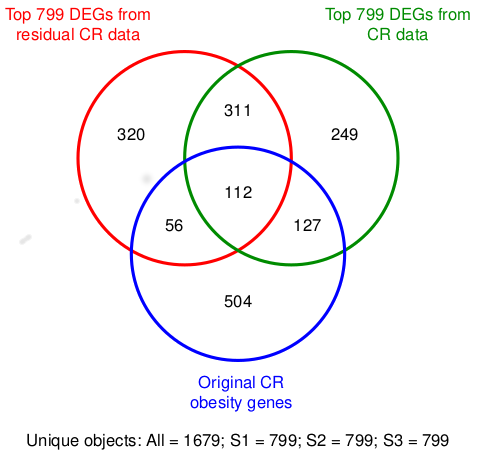
\includegraphics[width=0.5\linewidth]{results1/deg_venn1}
	\caption[Venn diagram of the \glspl{deg} identified from the CR data (all patients included)]{Venn diagram showing the common gene probes between the signatures obtained from the unadjusted and the clinical variable-adjusted CR data and the original obesity associated genetic signature from the \citet{Creighton2012} study }
	\label{fig:venn1}
\end{figure}

\noindent
There was a possible bias between the different ethnic groups, where African-American patients were more likely to be obese compared with the Caucasian patients (13 out of 16 were obese in African-American group, whereas 22 out of 77 were obese in Caucasian group; see \cref{ssub:creighton_study,tab:num_sample_microarray} in \cref{sub:breast_cancer_data}).
Though ethnicity was controlled in the residual CR data, the effect of ethnicity on the CR data was completely removed to prevent any possibility of ethnicity influencing the analysis.
Therefore, the effect of ethnicity was ignored by considering only the Caucasian patients in the CR data, which left a total of 77 Caucasian patients in the data set.

With the Caucasian-only CR data set, obesity associated genetic signatures were identified as described above.
% ; first in the unadjusted data, then in the data with clinical variables adjusted (except ethnicity, as it has already been controlled for by considering only the Caucasian samples), and lastly the common genes between each of these two signatures with the original obesity associated genetic signature were identified.
2129 and 1558 gene probes were significantly differentially expressed (unadjusted p-value \textless{} 0.01) in the unadjusted and clinical variable-adjusted Caucasian patient data, respectively (\cref{tab:ob_deg_summary}).
As before, the most significant 799 gene probes were selected from these gene probes.
There were 148 and 92 common gene probes with the original Creighton \textit{et al.} obesity associated genetic signatures and unadjusted or clinical variable-adjusted Caucasian patient data set, respectively.
Again, Venn diagram was used to summarise the genes identified from the Caucasian patient data set (\cref{fig:venn2}).

\begin{figure}[tb]
	\centering
	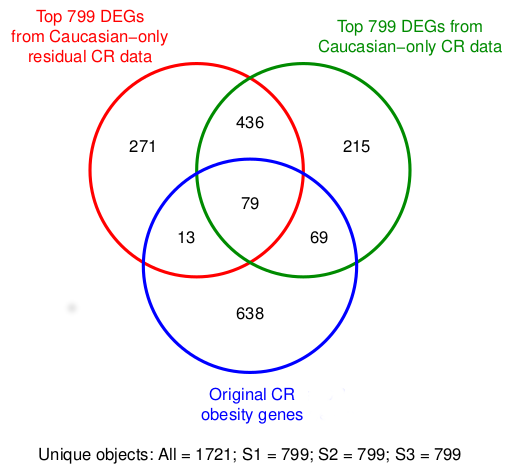
\includegraphics[width=0.5\linewidth]{results1/deg_venn2}
	\caption[Venn diagram of the \glspl{deg} identified from the CR data (Caucasian patients only)]{Venn diagram showing the common gene probes between the signatures obtained from the unadjusted and the clinical variable-adjusted CR data (Caucasian patients only) and the original obesity associated genetic signature from the \citet{Creighton2012} study}
	\label{fig:venn2}
\end{figure}

Additionally, the correlation of all of the obesity metagenes were examined to see whether these metagenes were similar to one another.
As clearly shown in \cref{fig:cr_meta_cor}, there were two distinct groups within the eight metagenes: the first group contained the obesity metagenes that were not overlapped with the Or metagene (Cr, Res, Ca and CaRes), while the other group had the overlapped metagenes (CrOl, ResOl, CaOl and CaResOl).
With that said, all eight metagenes showed high correlation with one another (lowest correlation approximately at 0.85), which suggested that all of these metagenes were detecting similar underlying biological mechanism from the data, as would be expected.

\begin{figure}[htpb]
	\centering
	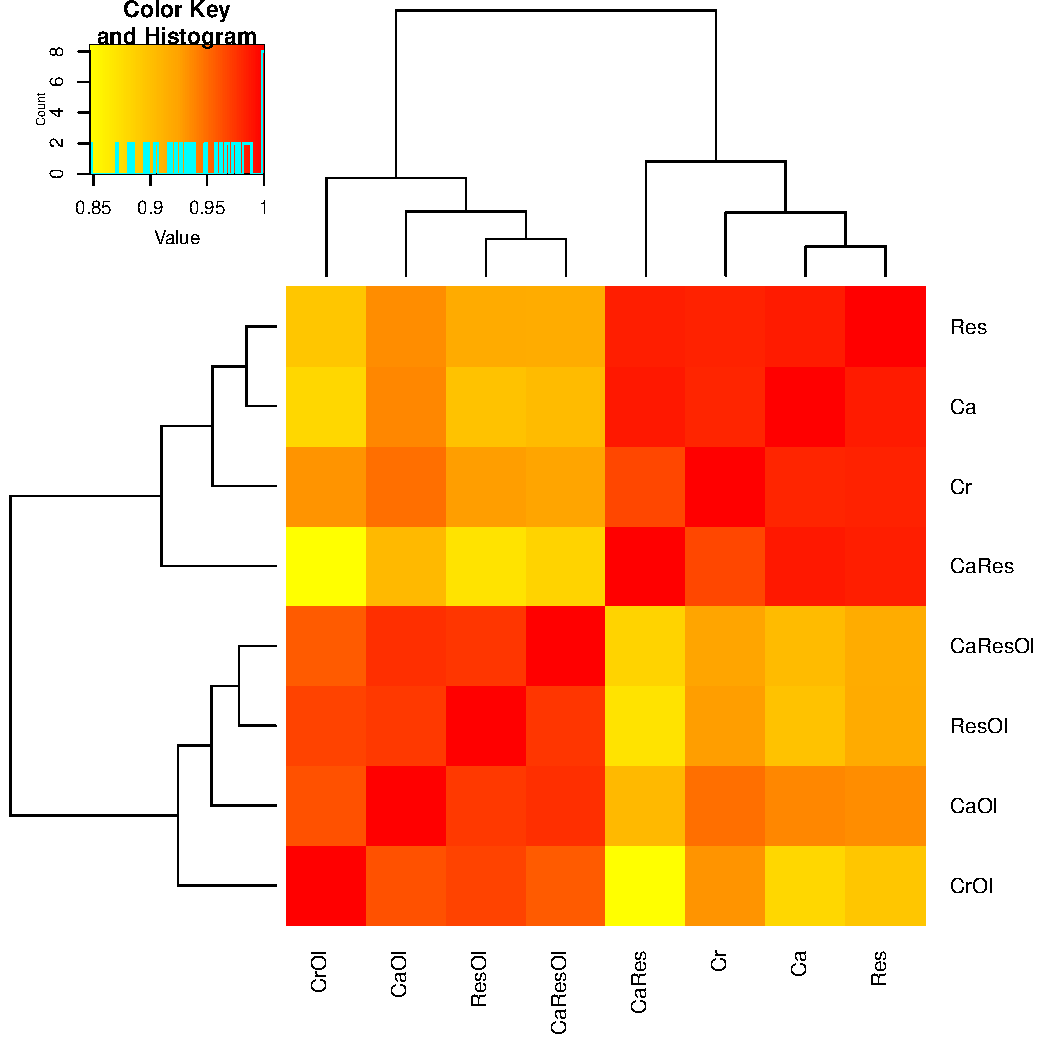
\includegraphics[width=0.8\linewidth]{results1/cr_meta_cor}
	\caption[Pearson correlation of all eight obesity metagenes identified in the CR data]{Heatmap showing the Pearson correlation of all eight obesity associated metagenes from the CR data with one another.
	\gls{svd} was applied to the \gls{rma} normalised CR data to generate each of the eight metagenes.
	High and low correlation were represented as red and blue, respectively, where the colours were matched with the values on the scale shown in the top right histogram.
	The lowest correlation was 0.8469, between the CrOl and the CaRes metagenes.
	}
	\label{fig:cr_meta_cor}
\end{figure}

Since all of these obesity associated genetic signatures were derived based on the discrete values of the patient \gls{bmi} status, an obesity associated genetic signature was searched for using the correlation of the gene probe expression with the patient \gls{bmi} value (continuous variable) in the CR data with all of the samples included, but no significant genes were identified (\cref{sec:obesity_associated_genetic_signature_using_sample_bmi_values}).
All of these obesity associated genetic signatures (eight in total) were checked to see whether these signatures had significant association with patient \gls{bmi} or \gls{bmi} status in the \gls{nzbc} and \gls{icgc} cancer data sets (\cref{sub:_novel_obesity_associated_signatures_and_sample_bmi}).
For simplicity, the abbreviations in \cref{tab:mg_abbrev} will be used to refer to the appropriate genetic signatures.

\begin{table}[tb]
	\centering
	\caption{Summary of the abbreviations used to refer to the different obesity associated genetic signatures identified in the CR data}
	\label{tab:mg_abbrev}
	\begin{tabular}{lp{0.51\textwidth}c}
		\hline
		\hline
		Abbreviation & Definition & No. of gene probes\\
		\hline
		\rule{0pt}{2.25ex}Or      & Original obesity associated genetic signature identified by \citet{Creighton2012}                       & 799\\
		\rule{0pt}{2.25ex}Cr      & Obesity associated genetic signature identified from unadjusted CR data                                & 799 \\
		\rule{0pt}{2.25ex}CrOl    & Genes common between Or and Cr genetic signatures                                                       & 239\\
		\rule{0pt}{2.25ex}Res     & Obesity associated genetic signature identified from clinical variable-adjusted CR data                & 799\\
		\rule{0pt}{2.25ex}ResOl   & Genes common between Or and Res genetic signatures                                                      & 168\\
		\rule{0pt}{2.25ex}Ca      & Obesity associated genetic signature identified from unadjusted Caucasian-only CR data                 & 799\\
		\rule{0pt}{2.25ex}CaOl    & Genes common between Or and Ca genetic signatures                                                       & 148\\
		\rule{0pt}{2.25ex}CaRes   & Obesity associated genetic signature identified from clinical variable-adjusted Caucasian-only CR data & 799\\
		\rule{0pt}{2.25ex}CaResOl & Genes common between Or and CaRes genetic signatures                                                    & 92\\
		\hline
		\hline
	\end{tabular}
\end{table}

\subsection{Novel obesity associated signatures and patient \gls{bmi}/\gls{bmi} status}
\label{sub:_novel_obesity_associated_signatures_and_sample_bmi}

As with the Or signature, all eight obesity associated genetic signatures were validated in the CR data set first, and then compared in other cancer data sets by using the transformation matrix that was generated in the \gls{rma} normalised CR data.
The CR data (unadjusted, all samples included) was normalised with the \gls{rma} method and \gls{svd} was applied to generate the all of the obesity metagenes.
The direction of the metagenes were examined to make sure that all of the metagenes were in line with one another (see \cref{sub:metagene_direction}; \cref{sec:direction_of_all_the_obesity_metagenes_from_the_cr_data}).
The comparison of the metagenes with the sample gene expression in the CR data were displayed as heatmaps (\cref{fig:degmetacr}; \cref{sec:rest_of_the_cr_ob_meta_heatmap_results_cr}).
It was clear from the heatmaps that all of the metagenes reflected the overall expression of the corresponding obesity associated genetic signatures.
The association of the metagenes with patient \gls{bmi} and \gls{bmi} status was significant for all eight of the obesity associated genetic signatures identified (\cref{fig:degmetacr}; \cref{sec:rest_of_the_cr_ob_meta_heatmap_results_cr}).
These results confirmed that all of the obesity associated genetic signatures identified in \cref{sub:identification_of_obesity_associated_genetic_signatures} significantly associated with patient \gls{bmi} and \gls{bmi} status in the CR data in which the metagenes were derived from.
In the \gls{nzbc} data, the higher the metagenes scores of the samples were, the more expressed the genes were (and vice versa), but lacked the association with the patient \gls{bmi} or \gls{bmi} status (\cref{fig:degmetaprint}; \cref{sec:rest_of_the_cr_ob_meta_heatmap_results_cris}).

\begin{figure}[htp!]
	\centering
	\includegraphics[page=3,width=0.8\linewidth]{results1/cr_deg_meta_vs_clin}\\
	\vspace{1em}
	\includegraphics[page=4,width=0.45\linewidth]{results1/cr_deg_meta_vs_clin}
	\hfill
	\includegraphics[page=5,width=0.45\linewidth]{results1/cr_deg_meta_vs_clin}
	\caption[Cr obesity metagene in the CR data]{Heatmap, scatter plot and box plot showing the association of the Cr obesity associated metagene with the sample gene expression, patient \gls{bmi} and \gls{bmi} status, respectively, from the CR data.
	The results for the other obesity metagenes are shown in \cref{sec:rest_of_the_cr_ob_meta_heatmap_results_cr}.
	Scales, p-values and $R^2$-value are as described in previous figures.}
	\label{fig:degmetacr}
\end{figure}

\begin{figure}[htp!]
	\centering
	\includegraphics[page=3,width=0.8\linewidth]{results1/cris_crdeg_trans_meta}\\
	\vspace{1em}
	\includegraphics[page=4,width=0.45\linewidth]{results1/cris_crdeg_trans_meta}
	\hfill
	\includegraphics[page=5,width=0.45\linewidth]{results1/cris_crdeg_trans_meta}
	\caption[Cr obesity metagene in the \gls{nzbc} data]{Heatmap, scatter plot and box plot showing the association of the Cr obesity associated metagene with the sample gene expression, patient \gls{bmi} and \gls{bmi} status, respectively, from the \gls{nzbc} data.
	The results for the other obesity metagenes are shown in \cref{sec:rest_of_the_cr_ob_meta_heatmap_results_cris}.
	Scales, p-values and $R^2$-value are as described in previous figures.}
	\label{fig:degmetaprint}
\end{figure}

To confirm whether these metagenes showed significant association with patient \gls{bmi} or \gls{bmi} status in other cancer types, the transformation matrix was applied to the \gls{icgc} cancer data.
In all of the \gls{icgc} cancer data sets, all eight metagene scores were reflective of the sample gene expression of the corresponding obesity associated genetic signatures (\cref{fig:degmetaicgc}; \cref{sec:rest_of_the_cr_icgc_cancer_heatmap_results}).
In all cancer types but \gls{blca}, none of the obesity metagenes significantly associated with the patient \gls{bmi} or \gls{bmi} status (\cref{sec:rest_of_the_cr_icgc_cancer_heatmap_results}).
As shown in \cref{fig:degmetaicgc}, the \gls{blca} data set showed significant association with the Cr metagene with the patient \gls{bmi} and \gls{bmi} status.
Furthermore, Res and Ca metagenes also showed statistical significance in the overweight group, \gls{anova} and the regression line p-values; CaRes and Res metagenes were significant in overweight group and \gls{anova} p-value; CrOl and CaResOl metagenes were significant in overweight group; and ResOl and CaOl metagenes were not significantly associated with the sample \gls{bmi} or \gls{bmi} status in \gls{blca} data set (summarised in \cref{tab:degmetablca}).

This was unexpected since all of the genetic signatures resulted from the  gene expression analysis between the non-obese group and the obese group of the samples in the CR data, and yet all of the obesity metagenes showed significant association with the overweight group rather than the obese group in the \gls{blca} data set.
These results suggested that the samples from the patients that were overweight in the \gls{blca} data were similar in genotype with the samples from the patients that were obese in the CR data.
Again, due to the fact that all of the metagenes lacked association with the patient \gls{bmi} and  \gls{bmi} status in all of the other \gls{icgc} cancer types, it was difficult to conclude whether the observed association of many of the obesity metagenes with the overweight group of the samples was truly reflective of the effect resulted from these metagenes.

Taken together, these results showed that, even though all of the obesity metagenes significantly associated with the patient \gls{bmi} and \gls{bmi} status in the original data where the genetic signatures were derived from, none of the metagenes were not generalisable in other cancer data sets.
Furthermore, these results showed that the lack of association with patient \gls{bmi} and \gls{bmi} status were not due to other clinical variables in the CR data set.
This raised a question of whether there was any obesity associated genetic signature that was common in multiple types of cancer (\cref{sec:common_genes_across_multiple_cancer_types}).

\begin{table}[htpb]
	\centering
	\caption{Statistics of all the obesity metagenes with the patient \gls{bmi} and \gls{bmi} status in the \gls{icgc} \gls{blca} cancer data}
	\label{tab:degmetablca}
	\begin{threeparttable}
		\begin{tabular}{lccccc}
			& \multicolumn{3}{c}{ P-values} & \multicolumn{2}{c}{ Regression line statistics}\\
			\cmidrule(r){2-4} \cmidrule(r){5-6}
			 Metagenes &  Overweight &  Obese &  \gls{anova} &  R$^2$ &  P \\
			\hline
			\hline
			\rule{0pt}{2.25ex}Cr & {\bfseries 0.0134}\tnote{1} & 0.1365 & {\bfseries 0.0387} & 0.0171 & {\bfseries 0.0195} \\
			Res                  & {\bfseries 0.0055}          & 0.1974 & {\bfseries 0.0196} & 0.0117 & {\bfseries 0.0446} \\
			CrOl                 & {\bfseries 0.0383}          & 0.4583 & 0.1096             & 0.0047 & 0.1374             \\
			ResOl                & 0.0909                      & 0.7092 & 0.2125             & 0.0018 & 0.2254             \\
			Ca                   & {\bfseries 0.0077}          & 0.1973 & {\bfseries 0.0231} & 0.0116 & {\bfseries 0.0456} \\
			CaRes                & {\bfseries 0.0104}          & 0.2712 & {\bfseries 0.0322} & 0.0101 & 0.0572             \\
			CaOl                 & 0.0575                      & 0.6185 & 0.1487             & 0.0022 & 0.2126             \\
			CaResOl              & {\bfseries 0.0463}          & 0.5820 & 0.1263             & 0.0036 & 0.1660             \\
			\hline
			\hline
		\end{tabular}
		\begin{tablenotes}
			\begin{footnotesize}
				\item [1] All values in bold are statistically significant (p \textless{} 0.05).
			\end{footnotesize}
		\end{tablenotes}
	\end{threeparttable}
\end{table}

\begin{figure}[htp!]
	\centering
	\includegraphics[page=3,width=0.8\linewidth]{results1/rawobsgene_ICGC}\\
	\vspace{1em}
	\includegraphics[page=4,width=0.45\linewidth]{results1/rawobsgene_ICGC}
	\hfill
	\includegraphics[page=5,width=0.45\linewidth]{results1/rawobsgene_ICGC}
	\caption[Cr obesity metagene in the \acrshort{icgc} \acrshort{blca} data]{Heatmap, scatter plot and box plot showing the association of the Cr obesity metagene with the sample gene expression, patient \gls{bmi} and \gls{bmi} status, respectively, from the \acrshort{icgc} \acrshort{blca} data.
	The results for other other metagenes and other \gls{icgc} cancer types are shown in \cref{sec:rest_of_the_cr_icgc_cancer_heatmap_results}.
	Scales, p-values and $R^2$-value are as described in previous figures.}
	\label{fig:degmetaicgc}
\end{figure}

\section{Common genes across multiple cancer types}
\label{sec:common_genes_across_multiple_cancer_types}

It was clear that the all of the obesity associated genetic signatures created from the CR data set were not significantly associated with patient \gls{bmi} across different \gls{icgc} cancer data sets.
To determine whether there was any obesity associated genetic signature that was expressed in multiple different cancer types, gene expression analysis was carried out on each of the eight \gls{icgc} cancer types, and common genes were searched from the \glspl{deg} that were identified.
All of the \gls{icgc} cancer data sets were normalised with voom (\cref{ssub:rna_seq_data}), which were then put through the gene expression analysis pipeline to identify the \glspl{deg} between the obese and non-obese groups of samples (\cref{sec:gene_expression_analysis}).
\cref{tab:icgcdegnum} summarised the number of \glspl{deg}  (unadjusted p \textless{} 0.05) found from each cancer type.

\begin{table}[tb]
	\centering
	\caption{Summary of the number of \glspl{deg} identified in each of the \gls{icgc} cancer data set}
	\label{tab:icgcdegnum}
	\begin{tabular}{lc}
		Cancer type & No. of \glspl{deg} identified\\
		\hline
		\hline
		\rule{0pt}{2.25ex}\gls{blca} & 679 \\
		\gls{cesc} & 1229\\
		\gls{coad} & 974\\
		\gls{kirp} & 687\\
		\gls{lihc} & 3340\\
		\gls{read} & 796\\
		\gls{skcm} & 1137\\
		\gls{ucec} & 2934\\
		\hline
		\hline
	\end{tabular}
\end{table}

There were 9695 unique \glspl{deg} across the eight different cancer types, and these genes were checked for any commonalities across the different cancer types.
There were 7330 genes that were differentially expressed in one cancer type, 2024 genes differentially expressed in any two cancer types, 320 genes expressed in any three cancer types, and 21 genes expressed in any four cancer types.
There were no genes differentially expressed by five or more cancer types (see \cref{tab:icgcdegtab} for a summary).
To confirm that these results were statistically significant, the gene expression analysis was repeated 1000 times for each cancer type after the samples were randomised in each analysis (see \cref{sub:sample_randomisation_in_simulation_analysis}).
The results from the simulation were summarised together with the earlier results in \cref{tab:icgcdegtab}.

The results from the simulation showed that, on average, 5732 genes were found to be differentially expressed in any single cancer type, 1057 in any two cancer types, 111 in any three cancer types, and 7 in any four cancer types.
Unfortunately, there were no \glspl{deg} expressed in all eight cancer types, which confirmed that there was no common genes that were differentially expressed between the samples that were obese and normal weight.
When the results from the \gls{icgc} gene expression analysis were compared with the simulation results, the number of \glspl{deg} found were statistically significant, as the numbers of genes identified exceeded the 95$^{th}$ percentile values for up to four cancer types.
This result confirmed that the \glspl{deg} from the \gls{icgc} cancer data were not identified by chance.
However, this also showed that many of the \glspl{deg} identified in the gene expression analysis of the cancer types were observed by chance, and that the majority of these genes were likely to be false positives.

\begin{table}[tb]
	\centering
	\begin{threeparttable}
		\caption{Summary of the number of \glspl{deg} identified by the gene expression analysis and simulation analysis in the \gls{icgc} cancer data}
		\label{tab:icgcdegtab}
		\begin{tabular}{>{\quad}lcccccccc}
			& \multicolumn{8}{c}{\small No. of cancer types expressing the \glspl{deg}\tnote{1}}\\
			& 1 & 2 & 3 & 4 & 5 & 6 & 7 & 8\\
			\hline
			\hline
			\rule{0pt}{2.25ex}\hspace{-1em}{\small Results from gene expression analysis} & 7330 & 2024 & 320 & 21 & 0 & 0 & 0 & 0 \\
			\hspace{-1em}{\small Results from the simulation:\tnote{2}}                       &      &      &     &    &   &   &   &   \\
			{\small Mean no. of \glspl{deg} identified}                                   & 5732 & 1057 & 111 & 7  & 0 & 0 & 0 & 0 \\
			{\small $95^{th}$ percentile}                                                 & 6965 & 1722 & 227 & 20 & 2 & 0 & 0 & 0 \\
			\hline
			\hline
		\end{tabular}
		\begin{tablenotes}
			\begin{footnotesize}
			\item [1] The numbers represent the number of cancer types a gene was expressed in.
			\item [2] The simulation was repeated 1000 times, each with randomised samples.
			\end{footnotesize}
		\end{tablenotes}
	\end{threeparttable}
\end{table}

\section{Pathways enriched in \gls{icgc} data sets}
\label{sec:pathways_enriched_in_icgc_data_sets}

To check whether there were any significant pathways enriched in any of the \gls{icgc} cancer data sets that were associated with obesity, pathway enrichment analysis was carried out on each cancer type separately and then all cancer types combined (\cref{sec:pathway_enrichment_analysis}).
Each cancer type was normalised with voom (\cref{ssub:rna_seq_data}) and pathway enrichment analysis was carried out as described in \cref{sec:pathway_enrichment_analysis}.

When the pathway enrichment analysis was carried out with the \gls{kegg} pathway database, only the ``ABC transporter'' pathway was significantly enriched (\gls{fdr}-adjusted p-value \textless{} 0.05) in the \gls{cesc} data, and no other pathways were enriched in any of the other \gls{icgc} cancer types (\cref{sec:pathways_significant_in_each_of_the_cancer_types}).
With the Reactome database, ``Phosphatase bond hydrolysis by NUDT proteins'' (in \gls{blca}) and ``Mitochondrial ABC transporters'' (in \gls{cesc}) were significantly enriched (\cref{sec:pathways_significant_in_each_of_the_cancer_types}).
With the \gls{go} database, there were 22 \gls{go} terms significantly enriched in \gls{blca}, 17 terms in \gls{cesc}, 3 terms in \gls{kirp}, 21 terms in \gls{read}, 10 terms in \gls{skcm}, 14 terms in \gls{ucec}, and no terms were significant in the \gls{coad} and \gls{lihc} cancer types (\cref{sec:pathways_significant_in_each_of_the_cancer_types}).

Though there were many \gls{go} terms identified as significantly enriched with the \gls{go} database in each of the cancer types, there were no terms that were common across all of the different cancer types.
Furthermore, these terms were not similar in terms of the biological activities involved.
For example, \gls{go} terms enriched in the \gls{blca} data suggested possible activation of the \gls{pi3k} pathway, but those enriched in the \gls{read} data were mainly involved in \acrshort{rna} processing (\cref{sec:pathways_significant_in_each_of_the_cancer_types}).
One interesting result from this enrichment analysis was that the ``ABC transport'' pathway was identified as significantly enriched in the \gls{cesc} data set by all three databases, suggesting that the ``ABC transport'' pathway may be a core component in the \gls{cesc} tumour biology.
All of these results indicated that the biological processes that drive tumour progression were unique to each cancer type, and no one pathway was associated with obesity and tumour biology across multiple cancer types.

Since there were no common pathway enriched in the \gls{icgc} cancer types when analysed individually, all of the \gls{icgc} cancer data sets were combined into a single data set to see any enriched pathways could be identified in a collective analysis.
The combined data set was generated in two ways.
The first combined data set was created by normalising (via voom) each cancer data set separately, combine all of the normalised cancer data sets into one, then applying batch correction to the data set (\cref{sub:batch_correction}).
The second combined data set was created by combining the cancer data sets into one big data set first, then the combined data was normalised, and finally batch correction was applied to obtain the final data set.
Each of the combined data sets were analysed for enriched pathways, but there were no pathways significantly enriched in either data sets.
These results suggested that there were no common biological pathways associated with obesity in the \gls{icgc} cancer data sets.

